\begin{document}

\chapter{Implementation}

In this chapter I will discuss how this project is structured, going through the high-level details of the actual implementation that respects all the requirements defined in Section \ref{Requirement Analysis}. It will review how the initial data is processed and how the extracted features of interest are used with a view to creating further synthetic datasets. Furthermore, the chapter examines how the Patchy-San algorithm operates on graph inputs in order to create suitable NNs training data and thus, how the NNs architectures are designed and optimised for the given classification task. Finally, the way in which files are renamed is analysed. 



\section{Overall Structure of the Project}

The renaming pipeline (clearly illustrated in Figure \ref{pipeline}) is comprised of four main components, each of them aiming to fulfil a different goal of the project:

\begin{itemize}
    \item \textbf{context classification pipeline:} this component is responsible with, firstly, generating synthetic graph datasets which mimic properties of real data. These graph are afterwards processed by the Patchy-San algorithm into suitable input for a convolutional neural network  which returns the desired predictions. Additionally, two off-the-shelf implementations of KNN and RandomForest algorithms were used as baseline for this component. 

    \item \textbf{content classification pipeline:} this component is responsible with, firstly, performing various transformations on log files content in order to obtain numerical vectors. These vectors are used as input for a multilayer perceptron, which returns the desired predictions.
    
    \item \textbf{ensemble of stacked classifiers:} the predictions obtained from the first two components are used (and hence, combined) to train and test a new ML model, a so-called meta-classifier. The final predictions of these stacking classifiers ensemble are regarded as the overall classification results. 
    
    \item \textbf{rule based renaming:} tacking into account the classification results, context information and a user-given policy, this component suggests renaming possibilities for files that have non-descriptive names. 
    
\end{itemize}

\begin{figure}[H]
  \centering
  \centerline{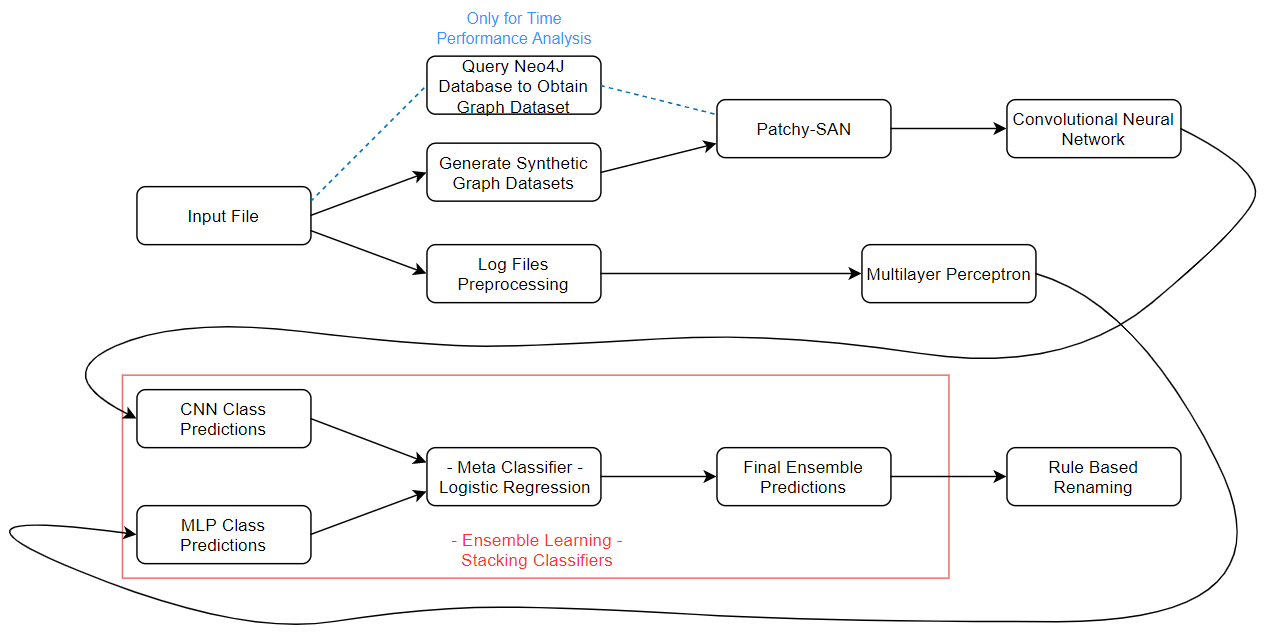
\includegraphics[scale = 0.5]{Images/pipeline.png}}
  \caption{Overview of the implemented ML pipeline.}
  \label{pipeline}
\end{figure}

Besides the renaming pipeline, the tuning and evaluation of the ML models was achieved using a popular procedure, nested cross-validation, which is described in detail in Section \ref{nested_cross_validation}. \\

When designing the ML models, a few of aspects have been taken into account: there is a lot of code that could be shared between the models and reused, the user would mostly be interested in model's functionality while implementation details could be hidden, and, the code should be highly scalable in that, at any time, a new model can be implemented and added to the project with ease. Given all of these, I decided to follow the object-oriented paradigm when building the classifiers. This design choice can be observed in Figure \ref{uml_oop}.

\section{Regularisation Techniques}

Deep NNs can be trained to develop complex relationships between their input data and their outcome. Depending on the amount of training data the network may develop a behaviour that brings good results for the training data, but fails as soon as unknown test data is fed into the network. To prevent overfitting in neural networks, there exist a variety of methods. A few of them were implemented and are discussed in this section.

\subsection{Weight Decay}
Weight decay$^{\small \cite{weight_decay}}$ is a standard trick to improve the generalisation performance of neural
networks by constraining the weights to be small in magnitude and penalising large weights. Specifically, weight decay is defined as multiplying each weight in the gradient descent at each epoch by a factor $\lambda$ smaller than one and greater than zero. This technique is equivalent to introducing an L2 regularisation term to the loss function that one wants to optimise. Therefore, the updated loss functions will be of the following form: 

\begin{equation} \label{weight_decay}
  \centering
  \mathfrak{L}_{updated} = \mathfrak{L}_{model} + \frac{\lambda}{2} \norm{\textbf{w}}
\end{equation} 

where $\norm{\textbf{w}} = \sqrt{\sum |w_i^2|}$ is the L2 norm of the weights vector.\smallskip

Keras provides a weight regularisation API that allows one to add a penalty for weight size to the loss function. A weight regularizer can be added to each layer when the layer is defined in a Keras model. This is achieved by setting the $kernel\_regularizer$ argument on each layer.

\begin{figure}[H]
  \centering
  \centerline{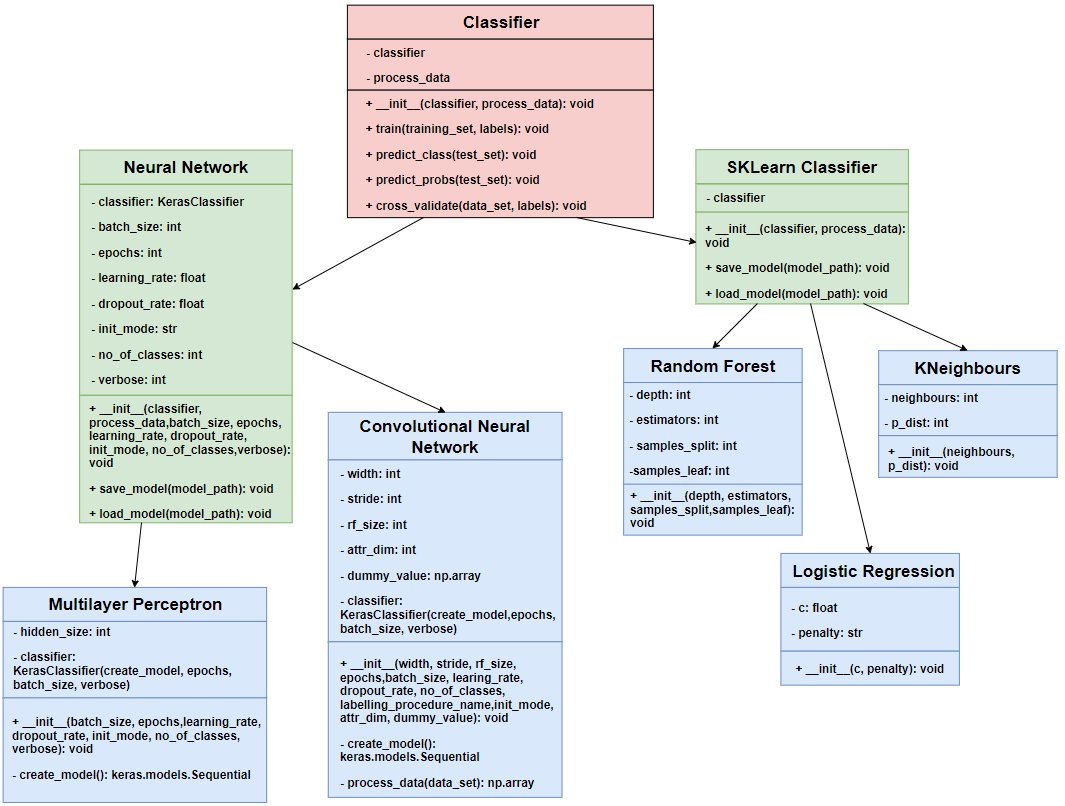
\includegraphics[scale = 0.6]{Images/uml.png}}
  \caption{UML diagram illustrating the inheritance of implemented classifiers.}
  \label{uml_oop}
\end{figure}

\subsection{Dropout}

Dropout$^{\small \cite{dropout}}$ is a regularisation technique behaving in the following manner: on each training iteration, a randomly chosen subset of neurons in the NN are shut down, in the sense that the NN will perform forward propagation and back-propagation as if those nodes (alongside with their inwards and outwards edges) are not preset at all. Since the units that are dropped out in each iteration are random, this forces the learning algorithm to spread out the weights and not focus on some specific features. This procedure can be visualised in Figure \ref{dropout}. In the simplest case, each unit is retained with a fixed probability $k_p$ independent of other units, which is introduced as a new hyperparameter in the NN. One important aspect to note is that the weights of the network will be larger than normal because of dropout. Thus, if a unit is retained with probability $k_p$ during training, the outgoing weights of that unit are multiplied by $k_p$ at test
time. Another approach is to re-scale weights at training time instead, after each weight update at the end of the mini-batch. This is sometimes called inverse dropout and is the way both Keras and Pytorch deep learning libraries implement it. 


\begin{figure}[H]
  \centering
 \centerline{ 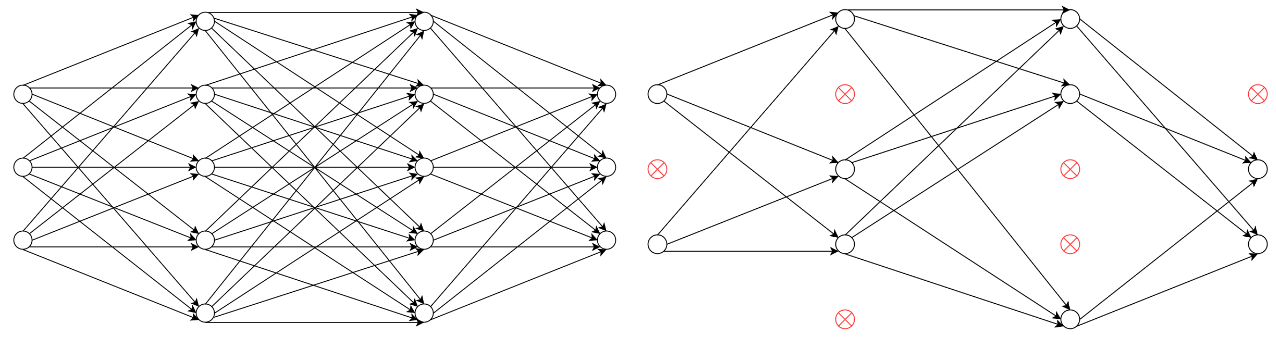
\includegraphics[scale = 0.5]{Images/dropout_new.png}}

  \caption{Neural Network before (LHS) and after (RHS) dropout.}
  \label{dropout}
\end{figure}

\subsection{Batch Normalisation}


One of the key motivations for the development of Batch Normalisation$^{\small \cite{batchnorm}}$ was the reduction of so-called internal covariate shift (ICS). ICS is the phenomenon wherein the distribution of inputs to a layer in the NN changes due to an update of parameters in the previous layers. This change leads to a constant shift of the underlying training problem and is thus believe to have detrimental effect on the training process. Therefore, Batch Normalisation is a mechanism that aims to stabilise the distribution (over a mini-batch) of inputs \{$x_1$, $x_2$, ... , $x_n$\} to a given NN during training. This is achieved by augmenting the NN with additional layers that set the first two moments: mean - $\mu = \frac{1}{n} \sum_{i=1}^n x_i$ and variance - $\sigma = \sqrt{\frac{1}{n} \sum_{i=1}^n (x_i - \mu) ^ 2}$, of the distribution of each activation to be zero and one respectively. Thus, it normalises the inputs in the following manner: 

\begin{equation}
  \centering
  \hat{x}_k = \frac{x_k - \mu}{\sqrt{\sigma + \epsilon}}
\end{equation}

where $\epsilon > 0$ is a small constant added to avoid division by 0. \smallskip

Then, the batch normalised inputs are also typically scaled and shifted based on trainable parameters $\gamma$ and $\beta$ to preserve model expressivity. 

\begin{equation}
  \centering
  y_k = \gamma_k * \hat{x}_k + \beta_k
\end{equation}

\subsection{Early Stopping}
A problem with training neural networks is in the choice of the number of training epochs to use. Too many epochs can lead to overfitting of the training dataset as well as high training times, whereas too few may result in an underfit model. Early stopping is a method that allows one to specify an arbitrary large number of training epochs and stop training once the model performance stops improving on a hold out validation dataset. The error on the validation set is used as a proxy for the generalisation error in determining when overfitting has begun (i.e. the moment that after achieving a minimum, the error on the validation set starts increasing again).\\

Keras supports the early stopping of training via a callback called EarlyStopping. This callback requires setting the performance measure to monitor (hence defining what is considered to be an improvement), the trigger, and once triggered, it will stop the training process. In Keras, callbacks provide a way to execute code and interact with the training model process automatically. Callbacks can be provided to the \textit{fit()} function via the \textit{callbacks} argument. Often, the first sign of no further improvement may not be the best time to stop training. This is because the model may coast into a plateau of no improvement or even get slightly worse before improving considerably. We can account for this by adding a delay to the trigger in terms of the number of epochs on which we would like to see no improvement. This can be done by setting the \textit{patience} argument. 


\section{Context Classification Pipeline}
\subsection{Data Analysis and Processing}

From the provenance graphs described in the introduction, the context classification algorithm will consider file, process, and socket nodes, alongside with some of their various properties, encoded either in integer or string format. The only processing step applied for nodes was removing the isolated ones. Relationships between nodes are generally represented by influence, directed, edges. The property of interest of an edge is its timestamp, which can be distributed across the nodes it connects. For nodes ending up with multiple timestaps from multiple edges, an average timestamp can be computed and used as a feature. Section \ref{node_seq_sel} explains the importance of this feature in the context classification pipeline. \\

Ideally, we would want for each file which needs to be classified to extract a sub-graph containing various processes and sockets interacting with it (not necessarily directly, i.e. in one hop) and use it as input for the ML pipeline. However, the provenance graphs are very sparse and this effect can be observed in Figure \ref{nodedegdist}. The total number of edges is roughly twice the total number of nodes (approximately 340,000 to 170,000). The problems raised by these aspects are further discussed and dealt with in Section \ref{Synthetic Data Generation} 


\begin{figure}[H]
  \centering
  \centerline{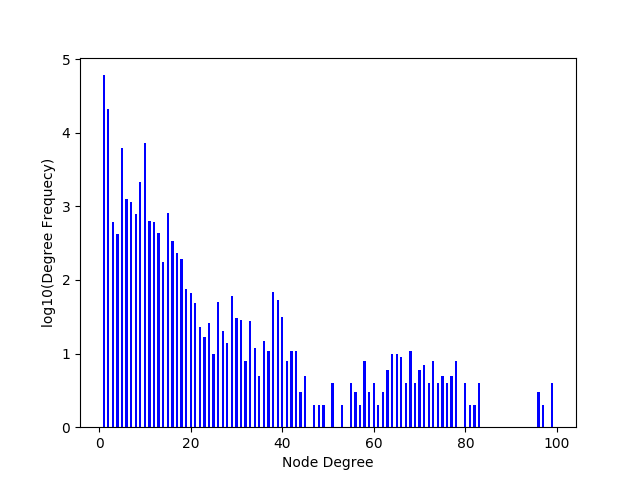
\includegraphics[scale = 0.7]{Images/nodedegdist.png}}
  \caption{Node degree distribution in Neo4J database.}
  \label{nodedegdist}
\end{figure}


\subsection{Feature Engineering}

There are 5 categorical features, in total, defining the feature vectors for each node: node$\_$type (file, process or socket), cmd$\_$line (for process), login$\_$user (for process), euid (for process), binary$\_$directory (for file). Note that although euid is an integer, it ranges in a very small set of values, which can be regarded as categories. \\


The major choice was between using integer or one-hot encoding for these features. The integer values have a natural ordered relationship between each other and machine learning algorithms may be able to understand and harness this relationship. For categorical variables where no such ordinal relationship exists, such as the ones present in this project, using integer encoding and allowing the model to assume a natural ordering between categories may result in poor performance or unexpected results. In this case, a one-hot encoding can be applied to the integer representation. This is where the integer encoded variable is removed and a new binary variable is added for each unique integer value. Only the N$_{th}$ binary variable is set to 1, when the integer representation is N. \\

For uniformity purposes, when one node does not present one of the features in the vector at all (e.g. a file does not have a cmd$\_$line), the feature is represented by the same number of binary variables, all 0. 

\subsection{Synthetic Data Generation} \label{Synthetic Data Generation}

Given the provenance data properties previously presented, it is simply not rich enough for conducting the intended experiments properly and creating a realistic view on the performance of the ML models. The aim of synthetic data generation is to create artificial datasets that mimic (some of) the properties of real data and are expressive enough to be successfully used for training and testing. 

\begin{figure}[H]
  \centering
  \centerline{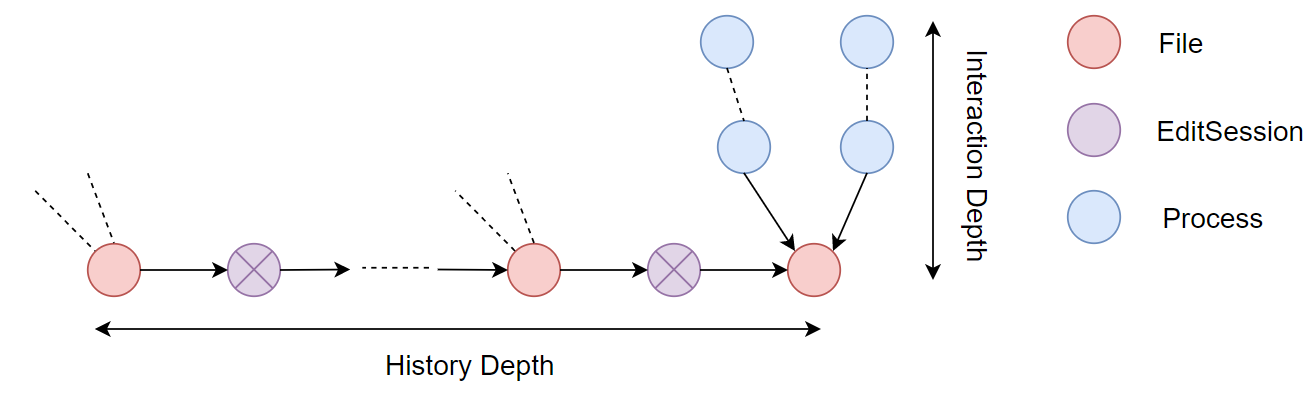
\includegraphics[scale = 0.35]{Images/synth_dataset.png}}
  \caption{Synthetic graph structure.}
  \label{synth_dataset}
\end{figure}

The most common pattern spotted in the real provenance data consists of a set of processes interacting with a file, the file then writing into an EditSession node all the changes made by the processes, and afterwards, and influence link is created between the EditSession and a new version of the file. This process is repeated multiple times, starting from the newly created version. An intuitive illustration is in Figure \ref{synth_dataset} (note that I decided to drop the EditSession nodes from the synthetic datasets as they are irrelevant for the actual classification). Given all of these, the properties on which generation of a synthetic graph is dependent are given below:

\begin{itemize}
    \item the node degree distribution of the real dataset
    \item the node type distribution of the real dataset (process, file, socket)
    \item the distributions of process properties: cmdline type, login$\_$user, euid value
    \item distributions of file properties: binary directory containing the file
    \item the number of versions of a file taken into account: History Depth (HD)
    \item the level of depth taken into account when it comes to processes interacting with the file: Interaction Depth (ID)
\end{itemize}

Ideally, we would like the distributions of process and file properties to be the main parameters that will differentiate between classes. \smallskip

Finally, the node timestamps are generated by assigning increasing numbers, in the following order: to the most recent version of the file, to the processes interacting with it (proportional to their ID), to older version of the file (proportional to their HD) and processes interacting with them. \smallskip

Before going through the highly complex processing step implemented by the Patchy-San algorithm, I must mention that the baseline models for context classification receive as input, for each graph, a list which contains the feature vectors of all nodes in the graph. \smallskip

\subsection{Patchy-San} \label{PCSN}

Patchy-San aims to bring CNNs to bear on a large-class of graph based learning problems. This novel algorithm consists of a general approach of extracting locally connected regions from graphs and model them in such a way so that they become a suitable input for a CNN. In this context, suitable refers to both structurally adequate and having the capability of preserving graph's expressivity, in the sense that local pattern information is not lost when linearising the set of features. 


\subsubsection*{Node Sequence Selection} \label{node_seq_sel}

The first step in the algorithm consists of establishing a node ordering for the input graph based on a chosen graph labelling function. In general, any reasonable graph labelling function would work for this sorting procedure. For instance, an artificial, independent of dataset knowledge approach, can use the betweenness centrality value of each node. However, given the insights into the provenance dataset, I tried to use the timestamp of the nodes for labelling purposes, as I thought it would imply a more natural ordering. Unfortunately, the results were substantially worse, and this might come from the fact that betweenness centrality conveys the structural information onto each node better that the ordering I tried to impose. In the end, I chose to stick with betweenness centrality. \\

Given this ordering, a subset of nodes is designated as the roots (Node Sequence) from where the actual receptive fields will be constructed. Specifically, each two consecutive picked roots from the sorted list of nodes are within a constant distance from each other. This distance ($s$) is called a stride. The aim is to construct the same $w$ number of receptive fields for each input graph as they will be provided as training/testing data for the convolutional neural network. Therefore, in case the number of nodes is not sufficient for building $w$ receptive fields, the algorithm creates all-zero receptive fields for padding purposes. 

\begin{figure}[H]
  \centering
  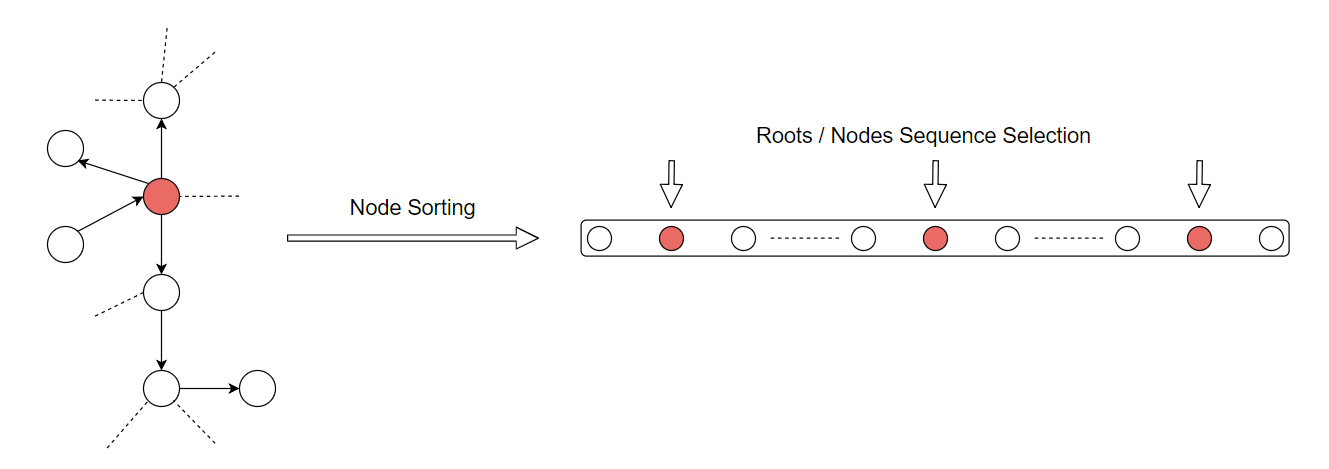
\includegraphics[scale=0.4]{Images/nodeseqsel.png}
  \caption{Input graph node's sorted with respect to the labelling function. $w$ root nodes selected within stride $s$.}
  \label{nodeseqsel}
\end{figure}

\subsubsection*{Neighbourhood Assembly}

The next stage involves assembling a local neighbourhood for each root previously determined. This is accomplished by using a standard breath-first search algorithm. Thus, I explore vertices with an increasing distance from the root, adding them to a set N. If the number of collected nodes is smaller than a pre-established number $k$, I continue exploring the immediate neighbours of the latest nodes added to the set until either $k$ nodes are found, or there are no more neighbours. In the latter case, for padding purposes, dummy nodes, having dummy attributes are added. This helps not throwing away information that might convey in-graph patters. However, it introduces the risk of misidentifying the padding nodes as a pattern themselves. \\

One final remark for the neighbourhood assembly procedure is that the order in which the immediate neighbours of a node are explored is with respect to, once again, the timestamp of each influence edge. Specifically, newer system activities will be considered with priority, also ensuring that the procedure is consistent and always gives the same output for the same graph. 

\begin{figure}[H]
  \centering
  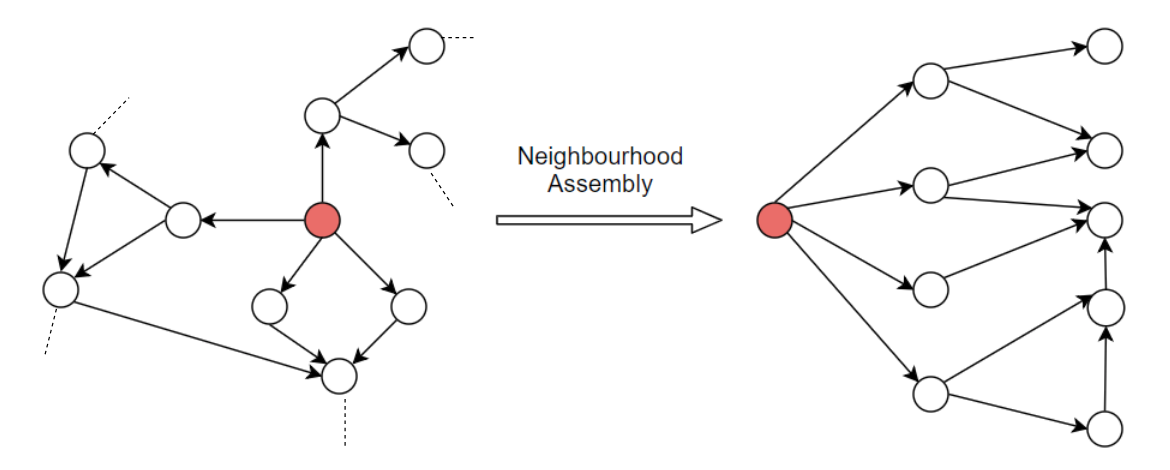
\includegraphics[scale=0.275]{Images/neighassemb2.png}
  \caption{Illustration of a Breath-First Search used for computing a neighbourhood.}
  \label{neighassemb}
\end{figure}


\subsubsection*{Receptive Field Normalisation}

The receptive field of a node is built by normalising the neighbourhood assembled in the previous step. The normalisation imposes an order on the nodes of the neighbourhood graph so as to map from the unordered graph space to a vector space with a linear order. This time, the graph labelling procedure is way more difficult to compute, as appropriately choosing it is at the core of the representation that Patchy-San proposes. Hence the performance of the classification pipeline will highly depend on the labelling procedure. \\

The basic idea is that the graph labelling procedure should assign nodes of two different graphs in similar positions if and only if they have similar structural roles in the graphs. The labelling of the vertices is therefore constrained by the graph distance to the root node $v$. For any two vertices $u$, $w$, if $u$ is closer to $v$ than $w$, then $v$ is
always ranked higher than $w$. This definition, illustrated in Figure \ref{normalisation}, ensures that $v$ has always rank 1, and that the closer a vertex is to $v$ in the graph, the higher it is ranked in the vector space representation. Consequently, in my project, this implies that groups of nodes denoting: processes interacting directly with the file to be classified, parent processes of the ones just mentioned, past processes interacting with the file at different moments in time; will be close together in the linear representation and also in same order for different graphs.

\begin{figure}[H]
  \centering
  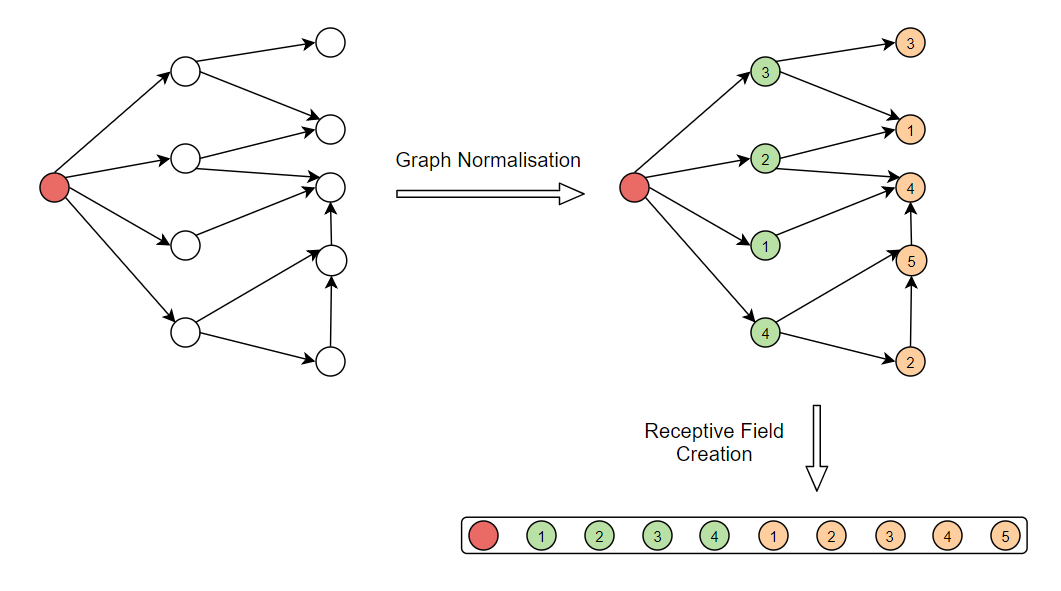
\includegraphics[scale=0.45]{Images/normalisation.png}
  \caption{Receptive Field Normalisation from previously selected neighbourhood. Nodes having the same colour have the same rank with respect to root in the liniarisation, while numbers illustrate tie-breakers.}
  \label{normalisation}
\end{figure}

One important detail that was taken into account is that, in general, the described labelling procedure does not consist of an injective function, thus a method to break ties between same-labelled nodes is necessary. In order to do so, and as suggested by the original paper of Patchy-San, I use pynauty, a python library which can be used to compare graphs for isomorphism and to determine their automorphism group. Pynauty$^{\small \cite{pynauty}}$ accepts prior node partitions as input (the subgraph neighbourhoods labelled w.r.t. distance to root node) and breaks remaining ties by choosing the lexicographically maximal adjacency matrix. Due to the constant size k of the neighborhood graphs, the graph isomorphism algorithm runs in time polynomial in the size of the original graph and, on average, in time linear in k. $^{\small \cite{timing_props}}$ 

\subsection{Convolutional Neural Network}

For each input graph $G$, given the construction of the receptive fields, and the number of attributes of each vertex $a_v$, I compute an initial 3D tensor of sizes ($w$, $k$, $a_v$), which is afterwards reshaped to a 2D tensor ($wk$, $a_v$) and fed as input for the CNN (where, obviously, $a_v$ will be the number of input channels). \\

The best CNN configuration that I found in my project consists of 7 layers. The input layer mentioned above. Two pairs of 1-dimensional convolutional and maxpooling layers after which the parameters are flattened. A fully connected layer and the output layer of probability distributions. The convolutional layers use 64 and 32 filters, respectively, while the pool size of the pooling layers is 2. \smallskip

After each of the pairs of convolutional and maxpooling, and also after the fully connected hidden layer, I add as regularisation techniques batch normalisation and dropout and as activation function ReLU. The output layer uses softmax activation function which returns the class probability distribution. \textit{He} model is used as the weights initialisation strategy, while weight decay at each hidden layer is used for penalising large weights. These layer-level operations can be visualised in Figure \ref{cnn_layers}. 

\begin{figure}[H]
  \centering
  \centerline{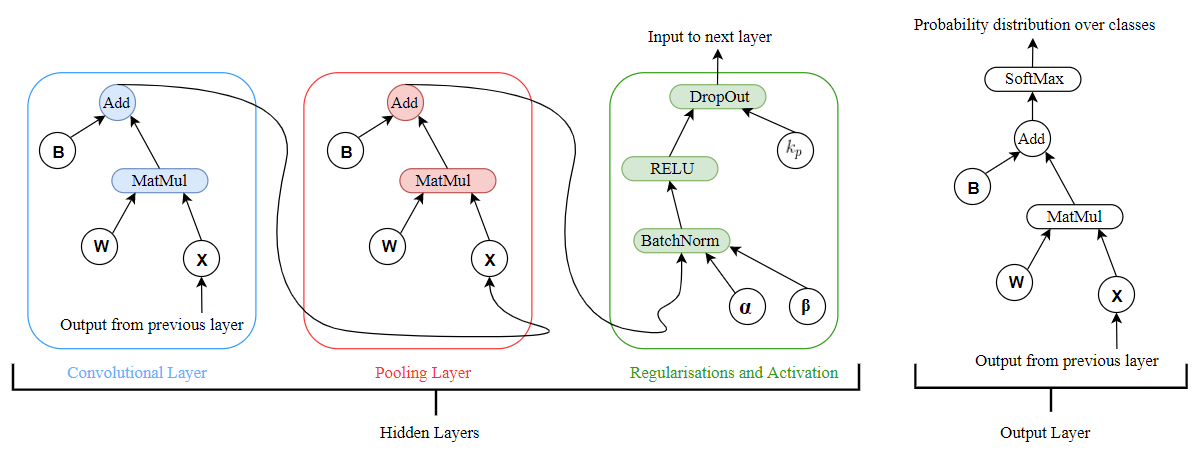
\includegraphics[scale=0.5]{Images/cnn_layers.png}}
  \caption{Diagram illustrating the configuration of hidden and output layers of the CNN.}
  \label{cnn_layers}
\end{figure}

Finally, the optimisation algorithm used is Adam$^{\small \cite{ADAM}}$ and the corresponding loss function is categorical crossentropy. Adam is a variation of gradient descent which leverages the power of adaptive learning rates methods to find individual learning rates for each parameter. An initial learning rate is still to be specified, but it alters and becomes less influential with each epoch depending on the parameter updated. This characteristic, combined with the fact that Adam only requires the computation of first-order gradients, usually makes it faster than other optimisers.  


\section{Content Classification Pipeline}
\subsection{Data Analysis and Processing}

The content component of the project was chosen with a view to proving the concept of combining both content and context information for classification purposes. The novelty of the project stands mostly in the Patchy-San-CNN pipeline, hence the content will not aim for generalisation, but rather for creating a bases for showing that further extensions are not only available, but also feasible. Bearing this in mind, I decided to approach a subcategory of files that can be present in provenance graphs: log files. The log files dataset does not match the actual nodes in the graphs for one main reasons: the project in which the provenance dataset was constructed happened more than one year ago, hence I did not have access to the content of those files. \\

Each log file in the dataset contains 100 lines of information. For each file, I concatenate all the lines in a single string and afterwards apply a couple of preprocessing steps to transform the string in numerical inputs for a NN. 

\subsubsection*{Feature Hashing}

Feature hashing$^{\small \cite{hashing_trick}}$ is a fast and space-efficient way of vectorising features. It works by converting unique tokens into integers. Specifically, by applying a hash function to the features and using their hash values as indices directly. It operates on the exact strings that one provides as input and does not perform any linguistic analysis or preprocessing. The advantage of using feature hashing is that text documents of variable-length, such as the involved log files, can be represented as numeric feature vectors of equal-length. This achieves at the same time a numerical input appropriate for machine learning algorithms, and also dimensionality reduction. Another aspect worth mentioning is that, for instance, in tasks involving natural language, it possible that some misspelling ends up incrementing the same index as some legitimate word as it passes through the hash function, resulting in a collision. This scenario is highly unlikely in my project, where the input consists of raw log files. Moreover, increasing the hash space dimensionality makes probability of collisions negligible.

\subsubsection*{Feature Scaling}

As previously mentioned, increasing the hash space has its upside in the fact that it reduces the probability of collisions. However, the larger the hash space the lower the ratio between the number of different values assigned to tokens over the number of different values provided by the hash function (given the constant content of the log files involved). These may result in the vectorised dataset containing features highly varying in magnitudes and range. Machine Learning algorithms usually don’t perform well when the input numerical attributes have very different scales. To suppress this effect, we need to bring all features to the same level of magnitudes. This can be achieved by scaling. \\

The scaling strategy applied in my project is called min-max scaling, in which values are
shifted and rescaled so that they end up ranging between 0 and 1. It is done by subtracting the min value and dividing by the max minus the min (min and max represent the minimum and maximum values in the feature vector X). The formal formula is given below: 

\begin{equation}
    \centering
    norm(X) = \frac{X - min(X)}{max(X) - min(X)}
\end{equation}

\subsection{Multilayer Perceptron}

The best architecture that I found for MLP for the log files classification task is comprised of four layers. The input layer consists of over 1000 neurons (length of the feature vector). The first hidden layer performs a significant reduction in that it has only 128 neurons. This decision is based on the fact that each additional layer increases the number of parameters the network has to optimise by \textit{O(mn)} for a transition from \textit{m} to \textit{n} neurons. The second hidden layer performs an expansion, having 256 neurons, and is meant to combine the features travelling through the network. The output layer consists of 6 neurons, giving the probability distribution of the input file being in each of the 6 classes. Each layer computes the weighed sum of its inputs and adds the bias. These process can be visualised in Figure \ref{mlp_layers} 

\begin{figure}[H]
  \centering
  \centerline{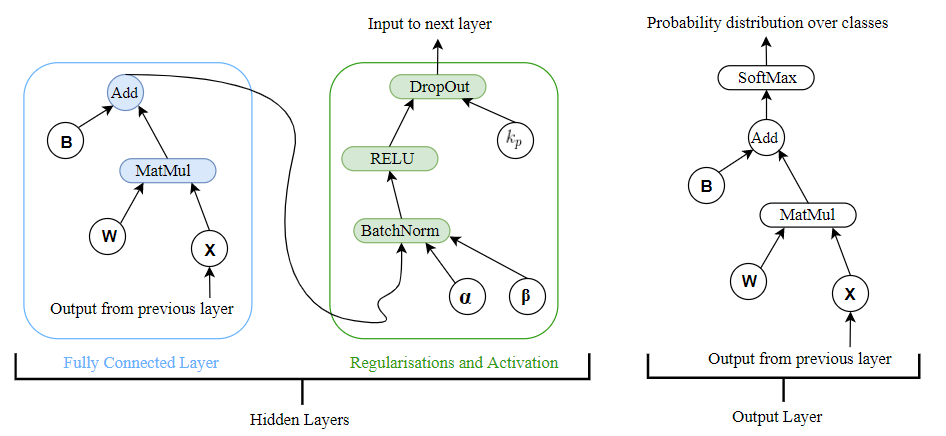
\includegraphics[scale=0.5]{Images/mlp_layers.png}}
  \caption{Diagram illustrating the configuration of hidden and output layers of the MLP.}
  \label{mlp_layers}
\end{figure}

In terms of regularisation techniques, I apply batch normalisation and dropout at each hidden layer, as well as early stopping monitoring validation loss, and \textit{He} model for initialising weights. Best results were found for dropout values with k$_p$ around 0.4, 0.5. Moreover, just like the CNN, the MLP optimises the parameters using the Adam algorithm and the categorical crossentropy loss function with weight decay regularisation (Equation \ref{weight_decay}). The ReLU function was chosen as the activation function for the neurons in the hidden layers of MLP, while for the output layer softmax activation function returns the desired probability distribution. 


\section{Ensemble Classification}

A successful approach to reducing the variance of neural network models is to train multiple models instead of a single model and to combine the predictions from these models. This is called ensemble learning and not only reduces the variance of predictions but also can (possibly) result in predictions that are better than any single model. 

\subsection{Stacking}

Stacking is an ensemble learning technique that combines multiple classification (or regression) models via a meta-classifier or a (meta-regressor). The base level models are trained based on a complete training set, then the meta-model is trained on the outputs of the base level models as features. The main aspect that makes this technique suitable for my project is that, in comparison with other ensemble learning methods (such as Bagging or Boosting$^{\small \cite{ensemble}}$), the base level of Stacking often consists of different learning algorithms. This makes possible combining the context and content features, which is at the core of the project.\\

In my implementation, I run a Nested Cross-Validation (described in Section \ref{nested_cross_validation}) over both CNN and MLP, and I concatenate their best predictions (i.e. predictions achieving highest accuracy score) over all ten outer folds, say $\{$CNN$_1$, CNN$_2$, ..., CNN$_N$$\}$ and $\{$MLP$_1$, MLP$_2$, ..., MLP$_N$$\}$ where N is the size of the files dataset. 
Afterwards I use a dataset obtained from pairing predictions from the two classifiers $\{$(CNN$_1$, MLP$_1$), (CNN$_2$, MLP$_2$), ..., (CNN$_N$, MLP$_N$)$\}$ and the original true labels for conducting a regular Cross-Validation on a meta-classifier. The outputs of the meta-classifier are regarded as the overall predictions of the entire implemented machine learning pipeline. My choice for a meta-classifier is Logistic Regression. 

\subsection{Logistic Regression}

Logistic Regression is one of the most simple and commonly used Machine Learning algorithms for two-class classification. It describes and estimates the relationship between one dependent binary variable and independent variables. A logistic regression will model the chance of an outcome based on individual characteristics. Because chance is a ratio, what will be actually modeled is the logarithm of the chance given by:: 

\begin{equation}
    \centering
    \text{logit($\pi$)} = \text{log}(\frac{\pi}{1 - \pi}) = \beta_0 + \beta_1 * X_1 + ... + \beta_n * X_n 
\end{equation} 

where $\pi$ indicates the probability of an event, and $\beta_i$ are the regression coefficients associated with the reference group and the $X_i$ explanatory variables. \\

In the multiclass case, in the settings of this project, the training algorithm uses the one-vs-all (OvA) scheme.
Build N(N-1) classifiers (for N classes), one classifier to distinguish each pair of classes $i$ and $j$. Let f$_{ij}$ be the classifier where class $i$ were positive examples and class $j$ were negative. Note f$_{ji}$ $=$ -f$_{ij}$. Classify using:

\begin{equation}
    \centering
    f(x) = \argmax_{i} \sum_{j} f_{ij}(x)
\end{equation} 

On the one hand, given of its efficient and straightforward nature, logistic regression doesn't require high computation power, it is easy to implement, easily interpretable and used widely by data analyst and scientist. On the other hand, logistic regression is not able to handle a large number of categorical features/variables. In these situations, it is vulnerable to overfitting. Logistic regression will not perform well with independent variables that are not correlated to the target variable and are very similar or correlated to each other. However, none of these properties are present in our case where the input consists of prediction labels from the base classifiers. Therefore, logistic regression is an excellent choice for a meta-classifier. 

\section{Nested Cross-Validation} \label{nested_cross_validation}

The fundamental success criteria of the project were to develop, tune and evaluate a ML pipeline capable of classifying files in term of both content and provenance data. In order to deal with the second and third mentioned goals, I have implemented a Nested Cross-Validation (CV) procedure$^{\small \cite{nested_cross_validation}}$. A detailed description of how it is performed follows and an expressive visualisation of it can be observed in Figure \ref{NestedCV}. 

\begin{itemize}[label={}]
  \item \textbf{Step 1.} divide the dataset into K stratified cross-validation folds at random
  \item \textbf{Step 2.} for each fold $k$ = 1,2,...,K (outer loop for evaluation of the model with selected hyperparameter):
        \begin{itemize}[label={}]
          \item 2.1. let fold $k$ be the outer test set
          \item 2.2. let all data except for fold $k$ be the outer training set
          \item 2.3. randomly split training set into L stratified fold
          \item 2.4. for each fold $l$ = 1,2,...,L (inner loop for hyperparameter tuning):
                \begin{itemize}[label={}]
                  \item 2.4.1. let fold $l$ be the inner validation set
                  \item 2.4.2. let all data except fold $k$ and fold $l$ be the inner training set
                  \item 2.4.3. train with each hyperparameter on inner training set and evaluate on fold $l$, keeping track of performance metrics
                \end{itemize}
          \item 2.5. for each hyperparameter setting, calculate average metrics score over the L folds and choose the best one
          \item 2.6. train a model with the best hyperparameter on fold $k$, evaluate its performance and save its score
        \end{itemize}
  \item \textbf{Step 3.} calculate the mean score over all K folds and report as the generalisation error
\end{itemize} 

An outer CV procedure is performed to provide a performance estimate used to select the optimal model. In each fold of the outer CV, the hyperparameters of the model are tuned independently to maximise an inner CV estimate of generalisation performance. The outer CV is then essentially estimating the performance of a method for fitting a model, CV based hyperparameter tuning. This eliminates the bias introduced by a flat CV procedure as the test data in each iteration of the outer CV has not been used to optimise the performance of the model in any way, and may therefore provide a more reliable criterion for choosing the best model. The computational expense of nested CV, however, is substantially higher. 


\begin{figure}[H]
  \centering
  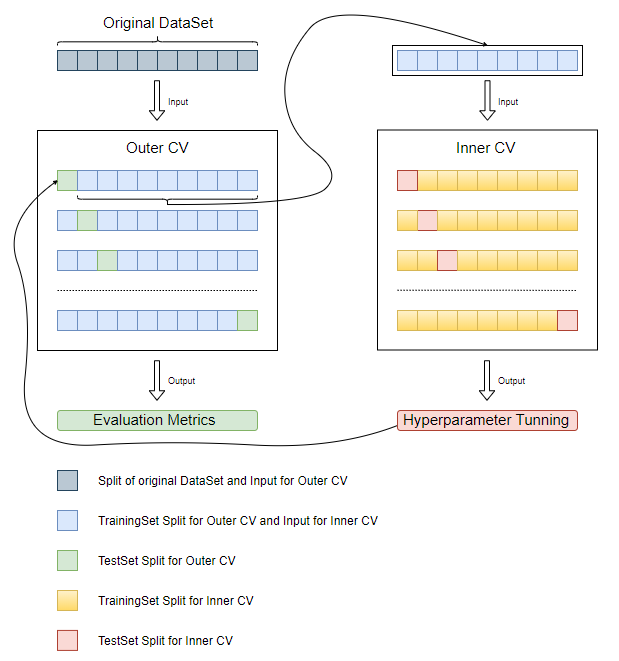
\includegraphics[scale=0.75]{Images/nested_cv.png}
  \caption{Structure of a Nested Cross-Validation used for both model evaluation and hyperparameter tuning.}
  \label{NestedCV}
\end{figure}

\section{Rule Based Renaming}

The renaming strategy applied in this project is purely rule based. It uses information from the provenance graphs of a file, alongside with the classification results. The user has the freedom to choose from a predefined set of properties that will serve as components in the newly created names. Specifically, a user can opt for using the class name and characteristics of processes that interact with the file (cmd$\_$line, login$\_$name, timestamp), in any combination. Finally, they can set a number of most recent processes to take into account. 

\section{Repository Overview}

The code repository is divided into three main modules: data processing and synthetic data generation (1), machine learning module (2) and evaluation module (3). Table \ref{repo_overview} goes into further detail, explaining at a fine-grained level, which pieces of functionality from each module were written from scratch and which are based on powerful libraries. 

\begin{longtable}{|p{.10\textwidth}||p{.15\textwidth}|p{.30\textwidth}|p{.45\textwidth}|}
  \hline
  \textbf{Module} & \textbf{Submodule} & \textbf{Functionality}                                                                                          & \textbf{Implementation Details}                                                                                                                \\
\hline
\noalign{\vspace{6pt}}
\hline

 \multirow{4}{*}{(1)}             & data loader        & loads into memory graph and log files.                                                                          & built from scratch.                                                                                                                             \\
\cline{2-4}
                  & synt data gen      & synthetic data generation w.r.t. parameters described in Section \ref{Synthetic Data Generation}.                & built from scratch.                                                                                                                            \\
\cline{2-4}
                  & neo4j driver       & classes achieving connection with the graph database and feature extraction capabilities.                        & built from scratch with the aid of neo4j driver library.                                                                                        \\
\cline{2-4}
                 & graph              & class of the graph objects processed by Patchy-San.                                                              & built from scratch with the aid of networkx library.                                                                                            \\
 \hline
\noalign{\vspace{6pt}}
\hline


 \multirow{6}{*}{(2)}              & patchy-san         & implements all the components of the patchy-san algorithm.                                                       & build from scratch except for the graph normalisation stage where pynauty is used for graph isomorphism implementation.                         \\
\cline{2-4}
                  & cnn                & implements convolutional neural network.                                                                         & network architecture built from scratch, while Keras API was used for the implementation of individual layers, activations and regularisations. \\
                \cline{2-4}

                 & mlp                & implements multilayer perceptron.                                                                                & architecture built from scratch, while Keras API was used for the implementation of individual layers, activations and regularisations. \\
                  \cline{2-4}

                   & rf                 & implements random forest classifier.                                                                             & used   sklearn.ensemble. RandomForestClassifier.                                                                                                \\
                \cline{2-4}
                  & knn                & implements k-nearest neighbours classifier.                                                                      & used sklearn.neighbors. KNeighborsClassifier.                                                                                                   \\
                \cline{2-4}
                 & lrg                & implements logistic regression classifier.                                                                       & sklearn.linear$\_$model.LogisticRegression.                                                                                                     \\

\hline
\noalign{\vspace{6pt}}
\hline

  \multirow{3}{*}{(3)}            & ncv                & implements a nested-cross validation.                                                                            & build from scratch to provide functionality for all implemented classifiers.                                                                    \\
\cline{2-4}
                   & permtest           & implements the Monte Carlo permutation test.                                                                     & built from scratch.                                                                                                                            \\
\cline{2-4}
                  & metrics            & defined the micro and macro metrics (Section \ref{Classification Metrics}) used for evaluation of ML algorithms. & implemented with the aid of sklearn.metrics.                                                                                                    \\


  \hline
  \caption[Repository Overview]{Implementation details of each module in the repository.}
  \label{repo_overview}
\end{longtable} 


\end{document}